\documentclass[10pt]{IEEEtran}

\usepackage{multicol}
\usepackage{cite}
\usepackage{amsmath,amssymb,amsfonts}
\usepackage{algorithmic}
\usepackage{graphicx}
\usepackage{textcomp}
% \usepackage{xcolor}
\usepackage[OT1]{fontenc} 
\usepackage{listings, listings-rust}
\usepackage{verbatim}
\usepackage[table]{xcolor}
\usepackage{float}

\definecolor{backcolour}{rgb}{0.93,0.93,0.93}
\lstdefinestyle{basicstyle}{
    backgroundcolor=\color{backcolour}
}

\lstset{style=basicstyle}

\begin{document}
\title{Rust vs C++: Performance in an extended sieve of Eratosthenes, and basic implementation of Chudnovsky algorithm}
\author{\IEEEauthorblockN{Zachary Meyner}
}
\date{}

\maketitle

\begin{abstract}
Rust is a young high performance programming language designed for safety and speed.
It's system of borrow checking at compile time ensures all code written in it is safe while keeping runtime high.
When considering the possibly of Rust for a project that requires high performance it is important to know how Rust compares to the traditionally fast programming langauges, specifically C and C++.
Many speed comparisons between the languages exist, but in this study we compare the speed of Rust and C++ in several Number Theory computations.
The results show that Rust is as fast or faster than C++ in our computations.
\end{abstract}
\section{Introduction}
Rust is a programming language maintained by Mozilla that is designed to maximize speed---in terms of time spent coding and 
execution---as well as safety. Rather than a garbage collector or manually managing memory safety of Rust is achieved 
through its system of ownership---a set of rules checked at compile time to ensure safety~\cite{rust2023}. The rules of ownership are:
\begin{itemize}
    \item Each value has an owner,
    \item Each value can only have one owner, and
    \item When the owner goes out of scope the variable is deleted~\cite{rust2023}.
\end{itemize}
Rust employs a system of borrowing for referencing. When a variable needs to be used in a different part of code, say a function, 
\begin{itemize}
    \item The variable is borrowed by that function via a reference and does not own that variable,
    \item The function cannot return that reference, and
    \item The reference is deleted at the end of the function call because of ownership~\cite{rust2023}.
\end{itemize}
Rust includes a very robust package manager, database, and build tool called “Cargo”~\cite{cargobook}. 
Cargo's package manager and repository--crates.io--makes community support for any features not included in the standard library to be maintained.
Rust's technology has allowed it to rank as the most popular language on Stack Overflow developer survey for seven years~\cite{stackoverflow2022}. 
The language has also amassed a large dedicated fanbase, including a discord server with 40,000+ users~\cite{discord}.
\par
Rust's potential in ease of writing in helped raise the popularity of the language and brought about speed tests of the language. 
It has been run against C in the embedded software and determined to be a viable alternative~\cite{BalasubramanianProceedings}. 
The safety benefits in systems programming has been explored~\cite{BalasubramanianProceedings}. 
Rust has also been compared to C, Fortran, and Java for speed and effort in parallel architectures, 
and found to be as fast as the fastest languages with the lowest amount of effort when programming~\cite{costanzo2021performance}\cite{heyman2020comparison}.
\par
The Sieve of Eratosthenes finds all prime numbers $p<n$ by starting at the first prime (normally 2) $p_0$ and multiplying by $k \leq \sqrt{n}$ where $k \in \mathbb{N}$ and marking resultant numbers as not prime.
When $k*p_0$ is done $\forall k$ the steps are repeated on the next unmarked number $p_1$.
The extended Sieve of Eratosthenes divides the range of the sieve into segments of size $\sqrt{n}+1$ and mark prime numbers in the respective ranges one segment at a time.
Dave Plummer has run a Sieve of Eratosthenes “race” on many programming languages\cite{plummer}. 
Plummer's results show a basic Sieve as opposed to an extended sieve, and rather than testing speed, Plummer tested how many times 
the sieve can go up to a number in a certain amount of time. 
The sieve of Eratosthenes gives an excellent test of the languages standard library vector implementations, and ease of writing array code in each langauge.
\par
Approximating $\pi$ has been one of the longest problems in Mathematics, dating back to Ancient Egypt\cite{burton}. Methods for approximating $\pi$ have become quite computationally efficient since then and eventually 
lead to a Ramunujan-type approximation by the Chudnovsky brothers which was used to break the the world record for computing $\pi$\cite{lynn}.
This numerical approximation provides a great way to compare the efficiency of Rust and C++, and external supported packages in each langauges.

\section{Methodology}
All tests were run 10 times on a local machine with a Xeon E5-2640 @2.40 GHz, 64 GB of RAM, running CentOS 9. The C++ complier is GCC 11.3.1 and the Rust complier is rustc 1.70.0-nightly (2023-03-28). All C++ builds will be using the \verb|-Ofast| 
compiler flag, and all rust builds will be done with the command \verb|cargo build --release| which by default 
uses the highest rustc speed optimization level\cite{cargobook}. For each program timing will be done via the linux \verb|/usr/bin/time| command to get the time at execution and once execution is done.
Each program will be run 10 times and have their execution times averaged together.
\subsection{Extended Sieve of Eratosthenes}
Input will determine the numeric limit for the sieve, and will start at 100,000,000.
After each programs has its time averaged for the given input, the input will increment by 500,000 and repeat the same process up to 500,000,000.
% The pseudocode outline used to code the sieve in both C++ and Rust is given:
% \begin{lstlisting}
% # Original sieve of Eratosthenes
% function sieve(vec &primes, u64 limit):
%     vec mark = [true; limit+1]
%     for even_entries in mark.step_by(2):
%         even_entries=false
% 
%     for i in (3..sqrt(limit)+1)
%              .step_by(2):
%         if mark[i]:
%             for j in (i*i..limit)
%                      .step_by(2*i):
%                 mark[j]=false
% 
%     for idx in (2..limit+1):
%         if mark[idx]:
%             primes.push(idx)
%             print(idx)
% 
% # Sieve extension
% function extended_sieve(u64 limit):
%     u64 size = sqrt(limit)+1
%     vec prime = vec[]
%     sieve(prime, size)
% 
%     u64 low = size+1
%     u64 high = 2*size
% 
%     while low < high:
%         if high > limit:
%             high = limit
%         
%         vec visited = [true; size+1]
% 
%         for val in prime:
%             u64 low_lim = (low/val)*val
% 
%             if low_lim < low:
%                 low_lim+=val
%             
%                 for j in (low_lim..high)
%                          .step_by(val):
%                     visited[j-low]=false
%         
%         for i in (low..high):
%             if visited[i-low]:
%                 print(i)
% 
%         low+=size
%         high+=size
% \end{lstlisting}
In both langauges the standard library vector and its associated functions were used.
For C++ that gives us \verb|std::vector<T>| and in Rust it is \verb|std::vec::Vec<T>| 
Rust's vector performs bound checking on calls, so 
it is better to use the langauges built in iterators in many places in 
the code. So C++ code such as:
\lstinputlisting[language=C++]{cppex.txt}
would be typed in Rust as:
\lstinputlisting[language=Rust]{rustex.txt}
This was done wherever possible to maximize the performance in Rust.
\subsection{Chudnovsky Algorithm}
Input size will determine how many digits of $\pi$ the programs will calculate, and will be starting at 50,000. 
After each programs time is averaged for the given input, the input will increment by 50,000 up to 250,000.
Chudnovsky algorithm will quickly exaust the precision possible by a 64-bit floating point number, as well as how large 64-bit integers can be, so big number packages will need to be used.
In both langauges the libraries gmp\cite{gmp} and mpfr\cite{mpfr} will be used for big numbers and big floats repsectively.
Since gmp and mpfr are C libraries they will work natively in C++, but for Rust we will need to use a library called ``rug'' from crates.io that acts as a wrapper to the C function calls\cite{rug}.
To get the rug library into the rust project we simply add \verb|rug = "1.19.1"| into the Cargo.toml file below the \verb|[dependencies]| line.
The use of community made wrapper for gmp leads to many changes in the code between the two, for example in C++ we have
\lstinputlisting[language=C++]{cppex2.txt}
which has the Rust equivalent of
\lstinputlisting[language=Rust]{rustext2.txt}
becuase of the rug library wrapper for gmp and mpfr.
\section{results}
\subsection{Extended Sieve of Eratosthenes}
\begin{table}[!ht]
    \centering
    \begin{tabular}{|c|cc|}
        \hline
        \rowcolor{lightgray}
            Input & Rust & C++ \\ \hline
            100000000 & 1.515 & 2.192 \\ 
            150000000 & 3.515 & 5.146 \\ 
            200000000 & 5.952 & 8.568 \\ 
            250000000 & 8.900 & 12.804 \\ 
            300000000 & 12.309 & 17.66 \\ 
            350000000 & 15.942 & 23.146 \\ 
            400000000 & 19.957 & 29.142 \\ 
            450000000 & 24.324 & 35.784 \\ 
            500000000 & 29.136 & 43.072\\ \hline
        \end{tabular}
    \caption{\label{sieve-table}Table comparison between Rust and C++ in an Extended Sieve of Eratosthenes}
\end{table}
As seen in Table~\ref{sieve-table} and Figure~\ref{sieve-graph} as input grows larger Rust becomes increasingly faster than C++.
\subsection{Chudnovsky Algorithm}
As seen in Figure~\ref{pi-graph} the speed of Chudnovsky is really close between Rust and C++, and Table~\ref{pi-table} shows that Rust is slighly faster than C++.
\begin{table}[!ht]
    \centering
    \begin{tabular}{|c|cc|}
        \hline
        \rowcolor{lightgray}
            Digits & Rust & C++ \\ \hline
            50000 & 41.525 & 55.47 \\ 
            100000 & 103.368 & 117.545 \\ 
            150000 & 265.303 & 280.494 \\ 
            200000 & 587.227 & 604.184 \\ 
            250000 & 1133.657 & 1153.602 \\ \hline
        \end{tabular}
    \caption{\label{pi-table}Table comparison between Rust and C++ in Chudnovsky Algorithm}
\end{table}
\begin{figure}[h]
    \centering
    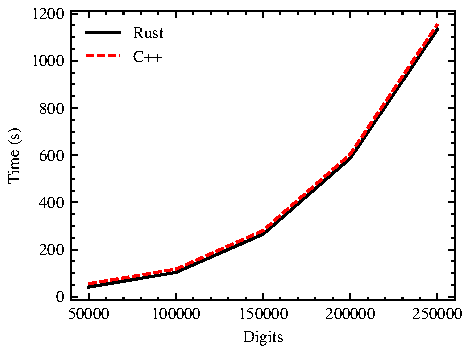
\includegraphics{piplot}
    \caption{\label{pi-graph}Graph comparison between Rust and C++ in Chudnovsky Algorithm}
\end{figure}
\begin{figure}[h]
    \centering
    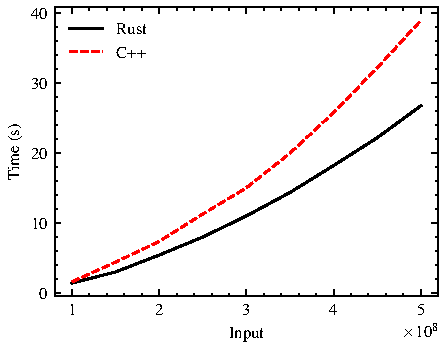
\includegraphics{sieveplot}
    \caption{\label{sieve-graph}Graph comparison between Rust and C++ in an Extended Sieve of Eratosthenes}
\end{figure}
\section{Discussion}
The results clearly show that Rust is able to calculate primes via the extended sieve significantly faster than C++, and is approximately equal to C++ in calculating digits of $\pi$ in the Chudnovsky algorithm.
We examined a calltree for the extended sieve program and were unable to determine what lead to the significant difference in execution time between the Rust and C++.
\section{Future Works}
Future works could look into what leads to the performance difference in extended sieve algorithm between the two langauges. Packages similar to GMP and MPFR could also be developed natively in Rust and tested against the speed of GMP and MPFR.\@
Addionally future works could look into the multithreaded performance of these algorithms in both languages.
\section{Conclusion}
In this study we showed that Rust is a potential alternative in terms of speed for numerical calculations-specifically the extended sieve and Chudnovsky Algorithm.
Rust performed significantly faster in an extended sieve of Eratosthenes and slighly faster than Chudnovsky algorithm in C++.
\nocite{*}
\bibliographystyle{IEEEtran}
\bibliography{propbib}
\end{document}
